%
% Statistics
%
\section{Statistics}

\subsection{deletedNodeAdditions}
deletedNodeAdditions is a statistic.

%
% value table of deletedNodeAdditions
%
\begin{tabular}{|l||l|}
\hline
	\textbf{Timestamp} & \textbf{Average} \\ \hline
	0 & 0 \\ \hline
	1 & 0 \\ \hline
	2 & 0 \\ \hline
	3 & 0 \\ \hline
	4 & 0 \\ \hline
	5 & 0 \\ \hline
	6 & 0 \\ \hline
	7 & 0 \\ \hline
	8 & 0 \\ \hline
	9 & 0 \\ \hline
	10 & 0 \\ \hline
	11 & 0 \\ \hline
	12 & 0 \\ \hline
	13 & 0 \\ \hline
	14 & 0 \\ \hline
	15 & 0 \\ \hline
	16 & 0 \\ \hline
	17 & 0 \\ \hline
	18 & 0 \\ \hline
	19 & 0 \\ \hline
	20 & 0 \\ \hline
	21 & 0 \\ \hline
	22 & 0 \\ \hline
	23 & 0 \\ \hline
	24 & 0 \\ \hline
	25 & 0 \\ \hline
	26 & 0 \\ \hline
	27 & 0 \\ \hline
	28 & 0 \\ \hline
	29 & 0 \\ \hline
	30 & 0 \\ \hline
	31 & 0 \\ \hline
	32 & 0 \\ \hline
	33 & 0 \\ \hline
	34 & 0 \\ \hline
	35 & 0 \\ \hline
	36 & 0 \\ \hline
	37 & 0 \\ \hline
	38 & 0 \\ \hline
	39 & 0 \\ \hline
	40 & 0 \\ \hline
	41 & 0 \\ \hline
	42 & 0 \\ \hline
	43 & 0 \\ \hline
	44 & 0 \\ \hline
	45 & 0 \\ \hline
\end{tabular}
\begin{tabular}{|l||l|}
\hline
	\textbf{Timestamp} & \textbf{Average} \\ \hline
	46 & 0 \\ \hline
	47 & 0 \\ \hline
	48 & 0 \\ \hline
	49 & 0 \\ \hline
	50 & 0 \\ \hline
\end{tabular}

\subsection{edgeWeightsToUpdate}
edgeWeightsToUpdate is a statistic.

See plot: \ref{plot:RANDOM_100_500 - BARABASI_ALBERT_GROWTH_10_2.z.statistics.updates.edges}, \ref{plot:RANDOM_100_500 - BARABASI_ALBERT_GROWTH_10_2.z.statistics.updates.edges.CDF}.

%
% value table of edgeWeightsToUpdate
%
\begin{tabular}{|l||l|}
\hline
	\textbf{Timestamp} & \textbf{Average} \\ \hline
	0 & 0 \\ \hline
	1 & 0 \\ \hline
	2 & 0 \\ \hline
	3 & 0 \\ \hline
	4 & 0 \\ \hline
	5 & 0 \\ \hline
	6 & 0 \\ \hline
	7 & 0 \\ \hline
	8 & 0 \\ \hline
	9 & 0 \\ \hline
	10 & 0 \\ \hline
	11 & 0 \\ \hline
	12 & 0 \\ \hline
	13 & 0 \\ \hline
	14 & 0 \\ \hline
	15 & 0 \\ \hline
	16 & 0 \\ \hline
	17 & 0 \\ \hline
	18 & 0 \\ \hline
	19 & 0 \\ \hline
	20 & 0 \\ \hline
	21 & 0 \\ \hline
	22 & 0 \\ \hline
	23 & 0 \\ \hline
	24 & 0 \\ \hline
	25 & 0 \\ \hline
	26 & 0 \\ \hline
	27 & 0 \\ \hline
	28 & 0 \\ \hline
	29 & 0 \\ \hline
	30 & 0 \\ \hline
	31 & 0 \\ \hline
	32 & 0 \\ \hline
	33 & 0 \\ \hline
	34 & 0 \\ \hline
	35 & 0 \\ \hline
	36 & 0 \\ \hline
	37 & 0 \\ \hline
	38 & 0 \\ \hline
	39 & 0 \\ \hline
	40 & 0 \\ \hline
	41 & 0 \\ \hline
	42 & 0 \\ \hline
	43 & 0 \\ \hline
	44 & 0 \\ \hline
	45 & 0 \\ \hline
\end{tabular}
\begin{tabular}{|l||l|}
\hline
	\textbf{Timestamp} & \textbf{Average} \\ \hline
	46 & 0 \\ \hline
	47 & 0 \\ \hline
	48 & 0 \\ \hline
	49 & 0 \\ \hline
	50 & 0 \\ \hline
\end{tabular}

\subsection{deletedEdgeRemovals}
deletedEdgeRemovals is a statistic.

%
% value table of deletedEdgeRemovals
%
\begin{tabular}{|l||l|}
\hline
	\textbf{Timestamp} & \textbf{Average} \\ \hline
	0 & 0 \\ \hline
	1 & 0 \\ \hline
	2 & 0 \\ \hline
	3 & 0 \\ \hline
	4 & 0 \\ \hline
	5 & 0 \\ \hline
	6 & 0 \\ \hline
	7 & 0 \\ \hline
	8 & 0 \\ \hline
	9 & 0 \\ \hline
	10 & 0 \\ \hline
	11 & 0 \\ \hline
	12 & 0 \\ \hline
	13 & 0 \\ \hline
	14 & 0 \\ \hline
	15 & 0 \\ \hline
	16 & 0 \\ \hline
	17 & 0 \\ \hline
	18 & 0 \\ \hline
	19 & 0 \\ \hline
	20 & 0 \\ \hline
	21 & 0 \\ \hline
	22 & 0 \\ \hline
	23 & 0 \\ \hline
	24 & 0 \\ \hline
	25 & 0 \\ \hline
	26 & 0 \\ \hline
	27 & 0 \\ \hline
	28 & 0 \\ \hline
	29 & 0 \\ \hline
	30 & 0 \\ \hline
	31 & 0 \\ \hline
	32 & 0 \\ \hline
	33 & 0 \\ \hline
	34 & 0 \\ \hline
	35 & 0 \\ \hline
	36 & 0 \\ \hline
	37 & 0 \\ \hline
	38 & 0 \\ \hline
	39 & 0 \\ \hline
	40 & 0 \\ \hline
	41 & 0 \\ \hline
	42 & 0 \\ \hline
	43 & 0 \\ \hline
	44 & 0 \\ \hline
	45 & 0 \\ \hline
\end{tabular}
\begin{tabular}{|l||l|}
\hline
	\textbf{Timestamp} & \textbf{Average} \\ \hline
	46 & 0 \\ \hline
	47 & 0 \\ \hline
	48 & 0 \\ \hline
	49 & 0 \\ \hline
	50 & 0 \\ \hline
\end{tabular}

\subsection{deletedEdgeWeightUpdates}
deletedEdgeWeightUpdates is a statistic.

%
% value table of deletedEdgeWeightUpdates
%
\begin{tabular}{|l||l|}
\hline
	\textbf{Timestamp} & \textbf{Average} \\ \hline
	0 & 0 \\ \hline
	1 & 0 \\ \hline
	2 & 0 \\ \hline
	3 & 0 \\ \hline
	4 & 0 \\ \hline
	5 & 0 \\ \hline
	6 & 0 \\ \hline
	7 & 0 \\ \hline
	8 & 0 \\ \hline
	9 & 0 \\ \hline
	10 & 0 \\ \hline
	11 & 0 \\ \hline
	12 & 0 \\ \hline
	13 & 0 \\ \hline
	14 & 0 \\ \hline
	15 & 0 \\ \hline
	16 & 0 \\ \hline
	17 & 0 \\ \hline
	18 & 0 \\ \hline
	19 & 0 \\ \hline
	20 & 0 \\ \hline
	21 & 0 \\ \hline
	22 & 0 \\ \hline
	23 & 0 \\ \hline
	24 & 0 \\ \hline
	25 & 0 \\ \hline
	26 & 0 \\ \hline
	27 & 0 \\ \hline
	28 & 0 \\ \hline
	29 & 0 \\ \hline
	30 & 0 \\ \hline
	31 & 0 \\ \hline
	32 & 0 \\ \hline
	33 & 0 \\ \hline
	34 & 0 \\ \hline
	35 & 0 \\ \hline
	36 & 0 \\ \hline
	37 & 0 \\ \hline
	38 & 0 \\ \hline
	39 & 0 \\ \hline
	40 & 0 \\ \hline
	41 & 0 \\ \hline
	42 & 0 \\ \hline
	43 & 0 \\ \hline
	44 & 0 \\ \hline
	45 & 0 \\ \hline
\end{tabular}
\begin{tabular}{|l||l|}
\hline
	\textbf{Timestamp} & \textbf{Average} \\ \hline
	46 & 0 \\ \hline
	47 & 0 \\ \hline
	48 & 0 \\ \hline
	49 & 0 \\ \hline
	50 & 0 \\ \hline
\end{tabular}

\subsection{randomSeed}
randomSeed is a statistic.

%
% value table of randomSeed
%
\begin{tabular}{|l||l|}
\hline
	\textbf{Timestamp} & \textbf{Average} \\ \hline
	0 & 1455542M \\ \hline
	1 & 1455542M \\ \hline
	2 & 1455542M \\ \hline
	3 & 1455542M \\ \hline
	4 & 1455542M \\ \hline
	5 & 1455542M \\ \hline
	6 & 1455542M \\ \hline
	7 & 1455542M \\ \hline
	8 & 1455542M \\ \hline
	9 & 1455542M \\ \hline
	10 & 1455542M \\ \hline
	11 & 1455542M \\ \hline
	12 & 1455542M \\ \hline
	13 & 1455542M \\ \hline
	14 & 1455542M \\ \hline
	15 & 1455542M \\ \hline
	16 & 1455542M \\ \hline
	17 & 1455542M \\ \hline
	18 & 1455542M \\ \hline
	19 & 1455542M \\ \hline
	20 & 1455542M \\ \hline
	21 & 1455542M \\ \hline
	22 & 1455542M \\ \hline
	23 & 1455542M \\ \hline
	24 & 1455542M \\ \hline
	25 & 1455542M \\ \hline
	26 & 1455542M \\ \hline
	27 & 1455542M \\ \hline
	28 & 1455542M \\ \hline
	29 & 1455542M \\ \hline
	30 & 1455542M \\ \hline
	31 & 1455542M \\ \hline
	32 & 1455542M \\ \hline
	33 & 1455542M \\ \hline
	34 & 1455542M \\ \hline
	35 & 1455542M \\ \hline
	36 & 1455542M \\ \hline
	37 & 1455542M \\ \hline
	38 & 1455542M \\ \hline
	39 & 1455542M \\ \hline
	40 & 1455542M \\ \hline
	41 & 1455542M \\ \hline
	42 & 1455542M \\ \hline
	43 & 1455542M \\ \hline
	44 & 1455542M \\ \hline
	45 & 1455542M \\ \hline
\end{tabular}
\begin{tabular}{|l||l|}
\hline
	\textbf{Timestamp} & \textbf{Average} \\ \hline
	46 & 1455542M \\ \hline
	47 & 1455542M \\ \hline
	48 & 1455542M \\ \hline
	49 & 1455542M \\ \hline
	50 & 1455542M \\ \hline
\end{tabular}

\subsection{nodesToAdd}
nodesToAdd is a statistic.

See plot: \ref{plot:RANDOM_100_500 - BARABASI_ALBERT_GROWTH_10_2.z.statistics.updates.nodes}, \ref{plot:RANDOM_100_500 - BARABASI_ALBERT_GROWTH_10_2.z.statistics.updates.nodes.CDF}.

%
% value table of nodesToAdd
%
\begin{tabular}{|l||l|}
\hline
	\textbf{Timestamp} & \textbf{Average} \\ \hline
	0 & 0 \\ \hline
	1 & 10 \\ \hline
	2 & 10 \\ \hline
	3 & 10 \\ \hline
	4 & 10 \\ \hline
	5 & 10 \\ \hline
	6 & 10 \\ \hline
	7 & 10 \\ \hline
	8 & 10 \\ \hline
	9 & 10 \\ \hline
	10 & 10 \\ \hline
	11 & 10 \\ \hline
	12 & 10 \\ \hline
	13 & 10 \\ \hline
	14 & 10 \\ \hline
	15 & 10 \\ \hline
	16 & 10 \\ \hline
	17 & 10 \\ \hline
	18 & 10 \\ \hline
	19 & 10 \\ \hline
	20 & 10 \\ \hline
	21 & 10 \\ \hline
	22 & 10 \\ \hline
	23 & 10 \\ \hline
	24 & 10 \\ \hline
	25 & 10 \\ \hline
	26 & 10 \\ \hline
	27 & 10 \\ \hline
	28 & 10 \\ \hline
	29 & 10 \\ \hline
	30 & 10 \\ \hline
	31 & 10 \\ \hline
	32 & 10 \\ \hline
	33 & 10 \\ \hline
	34 & 10 \\ \hline
	35 & 10 \\ \hline
	36 & 10 \\ \hline
	37 & 10 \\ \hline
	38 & 10 \\ \hline
	39 & 10 \\ \hline
	40 & 10 \\ \hline
	41 & 10 \\ \hline
	42 & 10 \\ \hline
	43 & 10 \\ \hline
	44 & 10 \\ \hline
	45 & 10 \\ \hline
\end{tabular}
\begin{tabular}{|l||l|}
\hline
	\textbf{Timestamp} & \textbf{Average} \\ \hline
	46 & 10 \\ \hline
	47 & 10 \\ \hline
	48 & 10 \\ \hline
	49 & 10 \\ \hline
	50 & 10 \\ \hline
\end{tabular}

\subsection{nodesToRemove}
nodesToRemove is a statistic.

See plot: \ref{plot:RANDOM_100_500 - BARABASI_ALBERT_GROWTH_10_2.z.statistics.updates.nodes}, \ref{plot:RANDOM_100_500 - BARABASI_ALBERT_GROWTH_10_2.z.statistics.updates.nodes.CDF}.

%
% value table of nodesToRemove
%
\begin{tabular}{|l||l|}
\hline
	\textbf{Timestamp} & \textbf{Average} \\ \hline
	0 & 0 \\ \hline
	1 & 0 \\ \hline
	2 & 0 \\ \hline
	3 & 0 \\ \hline
	4 & 0 \\ \hline
	5 & 0 \\ \hline
	6 & 0 \\ \hline
	7 & 0 \\ \hline
	8 & 0 \\ \hline
	9 & 0 \\ \hline
	10 & 0 \\ \hline
	11 & 0 \\ \hline
	12 & 0 \\ \hline
	13 & 0 \\ \hline
	14 & 0 \\ \hline
	15 & 0 \\ \hline
	16 & 0 \\ \hline
	17 & 0 \\ \hline
	18 & 0 \\ \hline
	19 & 0 \\ \hline
	20 & 0 \\ \hline
	21 & 0 \\ \hline
	22 & 0 \\ \hline
	23 & 0 \\ \hline
	24 & 0 \\ \hline
	25 & 0 \\ \hline
	26 & 0 \\ \hline
	27 & 0 \\ \hline
	28 & 0 \\ \hline
	29 & 0 \\ \hline
	30 & 0 \\ \hline
	31 & 0 \\ \hline
	32 & 0 \\ \hline
	33 & 0 \\ \hline
	34 & 0 \\ \hline
	35 & 0 \\ \hline
	36 & 0 \\ \hline
	37 & 0 \\ \hline
	38 & 0 \\ \hline
	39 & 0 \\ \hline
	40 & 0 \\ \hline
	41 & 0 \\ \hline
	42 & 0 \\ \hline
	43 & 0 \\ \hline
	44 & 0 \\ \hline
	45 & 0 \\ \hline
\end{tabular}
\begin{tabular}{|l||l|}
\hline
	\textbf{Timestamp} & \textbf{Average} \\ \hline
	46 & 0 \\ \hline
	47 & 0 \\ \hline
	48 & 0 \\ \hline
	49 & 0 \\ \hline
	50 & 0 \\ \hline
\end{tabular}

\subsection{addedEdges}
addedEdges is a statistic.

See plot: \ref{plot:RANDOM_100_500 - BARABASI_ALBERT_GROWTH_10_2.z.statistics.updates.edges}, \ref{plot:RANDOM_100_500 - BARABASI_ALBERT_GROWTH_10_2.z.statistics.updates.edges.CDF}.

%
% value table of addedEdges
%
\begin{tabular}{|l||l|}
\hline
	\textbf{Timestamp} & \textbf{Average} \\ \hline
	0 & 0 \\ \hline
	1 & 20 \\ \hline
	2 & 20 \\ \hline
	3 & 20 \\ \hline
	4 & 20 \\ \hline
	5 & 20 \\ \hline
	6 & 20 \\ \hline
	7 & 20 \\ \hline
	8 & 20 \\ \hline
	9 & 20 \\ \hline
	10 & 20 \\ \hline
	11 & 20 \\ \hline
	12 & 20 \\ \hline
	13 & 20 \\ \hline
	14 & 20 \\ \hline
	15 & 20 \\ \hline
	16 & 20 \\ \hline
	17 & 20 \\ \hline
	18 & 20 \\ \hline
	19 & 20 \\ \hline
	20 & 20 \\ \hline
	21 & 20 \\ \hline
	22 & 20 \\ \hline
	23 & 20 \\ \hline
	24 & 20 \\ \hline
	25 & 20 \\ \hline
	26 & 20 \\ \hline
	27 & 20 \\ \hline
	28 & 20 \\ \hline
	29 & 20 \\ \hline
	30 & 20 \\ \hline
	31 & 20 \\ \hline
	32 & 20 \\ \hline
	33 & 20 \\ \hline
	34 & 20 \\ \hline
	35 & 20 \\ \hline
	36 & 20 \\ \hline
	37 & 20 \\ \hline
	38 & 20 \\ \hline
	39 & 20 \\ \hline
	40 & 20 \\ \hline
	41 & 20 \\ \hline
	42 & 20 \\ \hline
	43 & 20 \\ \hline
	44 & 20 \\ \hline
	45 & 20 \\ \hline
\end{tabular}
\begin{tabular}{|l||l|}
\hline
	\textbf{Timestamp} & \textbf{Average} \\ \hline
	46 & 20 \\ \hline
	47 & 20 \\ \hline
	48 & 20 \\ \hline
	49 & 20 \\ \hline
	50 & 20 \\ \hline
\end{tabular}

\subsection{deletedEdgeAdditions}
deletedEdgeAdditions is a statistic.

%
% value table of deletedEdgeAdditions
%
\begin{tabular}{|l||l|}
\hline
	\textbf{Timestamp} & \textbf{Average} \\ \hline
	0 & 0 \\ \hline
	1 & 0 \\ \hline
	2 & 0 \\ \hline
	3 & 0 \\ \hline
	4 & 0 \\ \hline
	5 & 0 \\ \hline
	6 & 0 \\ \hline
	7 & 0 \\ \hline
	8 & 0 \\ \hline
	9 & 0 \\ \hline
	10 & 0 \\ \hline
	11 & 0 \\ \hline
	12 & 0 \\ \hline
	13 & 0 \\ \hline
	14 & 0 \\ \hline
	15 & 0 \\ \hline
	16 & 0 \\ \hline
	17 & 0 \\ \hline
	18 & 0 \\ \hline
	19 & 0 \\ \hline
	20 & 0 \\ \hline
	21 & 0 \\ \hline
	22 & 0 \\ \hline
	23 & 0 \\ \hline
	24 & 0 \\ \hline
	25 & 0 \\ \hline
	26 & 0 \\ \hline
	27 & 0 \\ \hline
	28 & 0 \\ \hline
	29 & 0 \\ \hline
	30 & 0 \\ \hline
	31 & 0 \\ \hline
	32 & 0 \\ \hline
	33 & 0 \\ \hline
	34 & 0 \\ \hline
	35 & 0 \\ \hline
	36 & 0 \\ \hline
	37 & 0 \\ \hline
	38 & 0 \\ \hline
	39 & 0 \\ \hline
	40 & 0 \\ \hline
	41 & 0 \\ \hline
	42 & 0 \\ \hline
	43 & 0 \\ \hline
	44 & 0 \\ \hline
	45 & 0 \\ \hline
\end{tabular}
\begin{tabular}{|l||l|}
\hline
	\textbf{Timestamp} & \textbf{Average} \\ \hline
	46 & 0 \\ \hline
	47 & 0 \\ \hline
	48 & 0 \\ \hline
	49 & 0 \\ \hline
	50 & 0 \\ \hline
\end{tabular}

\subsection{memory}
memory is a statistic.

See plot: \ref{plot:RANDOM_100_500 - BARABASI_ALBERT_GROWTH_10_2.z.statistics.memory}.

%
% value table of memory
%
\begin{tabular}{|l||l|}
\hline
	\textbf{Timestamp} & \textbf{Average} \\ \hline
	0 & 6.564 \\ \hline
	1 & 8.636 \\ \hline
	2 & 10.26 \\ \hline
	3 & 7.7 \\ \hline
	4 & 7.045 \\ \hline
	5 & 7.284 \\ \hline
	6 & 7.523 \\ \hline
	7 & 7.737 \\ \hline
	8 & 7.96 \\ \hline
	9 & 8.216 \\ \hline
	10 & 8.515 \\ \hline
	11 & 8.815 \\ \hline
	12 & 9.078 \\ \hline
	13 & 9.366 \\ \hline
	14 & 9.766 \\ \hline
	15 & 5.714 \\ \hline
	16 & 6.037 \\ \hline
	17 & 6.414 \\ \hline
	18 & 6.79 \\ \hline
	19 & 7.163 \\ \hline
	20 & 7.582 \\ \hline
	21 & 7.95 \\ \hline
	22 & 8.401 \\ \hline
	23 & 8.878 \\ \hline
	24 & 9.339 \\ \hline
	25 & 9.747 \\ \hline
	26 & 5.864 \\ \hline
	27 & 6.329 \\ \hline
	28 & 6.827 \\ \hline
	29 & 7.381 \\ \hline
	30 & 7.928 \\ \hline
	31 & 8.49 \\ \hline
	32 & 8.986 \\ \hline
	33 & 9.543 \\ \hline
	34 & 5.74 \\ \hline
	35 & 6.384 \\ \hline
	36 & 6.963 \\ \hline
	37 & 7.614 \\ \hline
	38 & 8.254 \\ \hline
	39 & 8.907 \\ \hline
	40 & 9.581 \\ \hline
	41 & 5.771 \\ \hline
	42 & 6.511 \\ \hline
	43 & 7.25 \\ \hline
	44 & 7.906 \\ \hline
	45 & 8.64 \\ \hline
\end{tabular}
\begin{tabular}{|l||l|}
\hline
	\textbf{Timestamp} & \textbf{Average} \\ \hline
	46 & 9.468 \\ \hline
	47 & 10.19 \\ \hline
	48 & 6.505 \\ \hline
	49 & 7.335 \\ \hline
	50 & 8.081 \\ \hline
\end{tabular}

\subsection{edgesToRemove}
edgesToRemove is a statistic.

See plot: \ref{plot:RANDOM_100_500 - BARABASI_ALBERT_GROWTH_10_2.z.statistics.updates.edges}, \ref{plot:RANDOM_100_500 - BARABASI_ALBERT_GROWTH_10_2.z.statistics.updates.edges.CDF}.

%
% value table of edgesToRemove
%
\begin{tabular}{|l||l|}
\hline
	\textbf{Timestamp} & \textbf{Average} \\ \hline
	0 & 0 \\ \hline
	1 & 0 \\ \hline
	2 & 0 \\ \hline
	3 & 0 \\ \hline
	4 & 0 \\ \hline
	5 & 0 \\ \hline
	6 & 0 \\ \hline
	7 & 0 \\ \hline
	8 & 0 \\ \hline
	9 & 0 \\ \hline
	10 & 0 \\ \hline
	11 & 0 \\ \hline
	12 & 0 \\ \hline
	13 & 0 \\ \hline
	14 & 0 \\ \hline
	15 & 0 \\ \hline
	16 & 0 \\ \hline
	17 & 0 \\ \hline
	18 & 0 \\ \hline
	19 & 0 \\ \hline
	20 & 0 \\ \hline
	21 & 0 \\ \hline
	22 & 0 \\ \hline
	23 & 0 \\ \hline
	24 & 0 \\ \hline
	25 & 0 \\ \hline
	26 & 0 \\ \hline
	27 & 0 \\ \hline
	28 & 0 \\ \hline
	29 & 0 \\ \hline
	30 & 0 \\ \hline
	31 & 0 \\ \hline
	32 & 0 \\ \hline
	33 & 0 \\ \hline
	34 & 0 \\ \hline
	35 & 0 \\ \hline
	36 & 0 \\ \hline
	37 & 0 \\ \hline
	38 & 0 \\ \hline
	39 & 0 \\ \hline
	40 & 0 \\ \hline
	41 & 0 \\ \hline
	42 & 0 \\ \hline
	43 & 0 \\ \hline
	44 & 0 \\ \hline
	45 & 0 \\ \hline
\end{tabular}
\begin{tabular}{|l||l|}
\hline
	\textbf{Timestamp} & \textbf{Average} \\ \hline
	46 & 0 \\ \hline
	47 & 0 \\ \hline
	48 & 0 \\ \hline
	49 & 0 \\ \hline
	50 & 0 \\ \hline
\end{tabular}

\subsection{addedNodes}
addedNodes is a statistic.

See plot: \ref{plot:RANDOM_100_500 - BARABASI_ALBERT_GROWTH_10_2.z.statistics.updates.nodes}, \ref{plot:RANDOM_100_500 - BARABASI_ALBERT_GROWTH_10_2.z.statistics.updates.nodes.CDF}.

%
% value table of addedNodes
%
\begin{tabular}{|l||l|}
\hline
	\textbf{Timestamp} & \textbf{Average} \\ \hline
	0 & 0 \\ \hline
	1 & 10 \\ \hline
	2 & 10 \\ \hline
	3 & 10 \\ \hline
	4 & 10 \\ \hline
	5 & 10 \\ \hline
	6 & 10 \\ \hline
	7 & 10 \\ \hline
	8 & 10 \\ \hline
	9 & 10 \\ \hline
	10 & 10 \\ \hline
	11 & 10 \\ \hline
	12 & 10 \\ \hline
	13 & 10 \\ \hline
	14 & 10 \\ \hline
	15 & 10 \\ \hline
	16 & 10 \\ \hline
	17 & 10 \\ \hline
	18 & 10 \\ \hline
	19 & 10 \\ \hline
	20 & 10 \\ \hline
	21 & 10 \\ \hline
	22 & 10 \\ \hline
	23 & 10 \\ \hline
	24 & 10 \\ \hline
	25 & 10 \\ \hline
	26 & 10 \\ \hline
	27 & 10 \\ \hline
	28 & 10 \\ \hline
	29 & 10 \\ \hline
	30 & 10 \\ \hline
	31 & 10 \\ \hline
	32 & 10 \\ \hline
	33 & 10 \\ \hline
	34 & 10 \\ \hline
	35 & 10 \\ \hline
	36 & 10 \\ \hline
	37 & 10 \\ \hline
	38 & 10 \\ \hline
	39 & 10 \\ \hline
	40 & 10 \\ \hline
	41 & 10 \\ \hline
	42 & 10 \\ \hline
	43 & 10 \\ \hline
	44 & 10 \\ \hline
	45 & 10 \\ \hline
\end{tabular}
\begin{tabular}{|l||l|}
\hline
	\textbf{Timestamp} & \textbf{Average} \\ \hline
	46 & 10 \\ \hline
	47 & 10 \\ \hline
	48 & 10 \\ \hline
	49 & 10 \\ \hline
	50 & 10 \\ \hline
\end{tabular}

\subsection{updatedEdgeWeights}
updatedEdgeWeights is a statistic.

See plot: \ref{plot:RANDOM_100_500 - BARABASI_ALBERT_GROWTH_10_2.z.statistics.updates.edges}, \ref{plot:RANDOM_100_500 - BARABASI_ALBERT_GROWTH_10_2.z.statistics.updates.edges.CDF}.

%
% value table of updatedEdgeWeights
%
\begin{tabular}{|l||l|}
\hline
	\textbf{Timestamp} & \textbf{Average} \\ \hline
	0 & 0 \\ \hline
	1 & 0 \\ \hline
	2 & 0 \\ \hline
	3 & 0 \\ \hline
	4 & 0 \\ \hline
	5 & 0 \\ \hline
	6 & 0 \\ \hline
	7 & 0 \\ \hline
	8 & 0 \\ \hline
	9 & 0 \\ \hline
	10 & 0 \\ \hline
	11 & 0 \\ \hline
	12 & 0 \\ \hline
	13 & 0 \\ \hline
	14 & 0 \\ \hline
	15 & 0 \\ \hline
	16 & 0 \\ \hline
	17 & 0 \\ \hline
	18 & 0 \\ \hline
	19 & 0 \\ \hline
	20 & 0 \\ \hline
	21 & 0 \\ \hline
	22 & 0 \\ \hline
	23 & 0 \\ \hline
	24 & 0 \\ \hline
	25 & 0 \\ \hline
	26 & 0 \\ \hline
	27 & 0 \\ \hline
	28 & 0 \\ \hline
	29 & 0 \\ \hline
	30 & 0 \\ \hline
	31 & 0 \\ \hline
	32 & 0 \\ \hline
	33 & 0 \\ \hline
	34 & 0 \\ \hline
	35 & 0 \\ \hline
	36 & 0 \\ \hline
	37 & 0 \\ \hline
	38 & 0 \\ \hline
	39 & 0 \\ \hline
	40 & 0 \\ \hline
	41 & 0 \\ \hline
	42 & 0 \\ \hline
	43 & 0 \\ \hline
	44 & 0 \\ \hline
	45 & 0 \\ \hline
\end{tabular}
\begin{tabular}{|l||l|}
\hline
	\textbf{Timestamp} & \textbf{Average} \\ \hline
	46 & 0 \\ \hline
	47 & 0 \\ \hline
	48 & 0 \\ \hline
	49 & 0 \\ \hline
	50 & 0 \\ \hline
\end{tabular}

\subsection{deletedNodeRemovals}
deletedNodeRemovals is a statistic.

%
% value table of deletedNodeRemovals
%
\begin{tabular}{|l||l|}
\hline
	\textbf{Timestamp} & \textbf{Average} \\ \hline
	0 & 0 \\ \hline
	1 & 0 \\ \hline
	2 & 0 \\ \hline
	3 & 0 \\ \hline
	4 & 0 \\ \hline
	5 & 0 \\ \hline
	6 & 0 \\ \hline
	7 & 0 \\ \hline
	8 & 0 \\ \hline
	9 & 0 \\ \hline
	10 & 0 \\ \hline
	11 & 0 \\ \hline
	12 & 0 \\ \hline
	13 & 0 \\ \hline
	14 & 0 \\ \hline
	15 & 0 \\ \hline
	16 & 0 \\ \hline
	17 & 0 \\ \hline
	18 & 0 \\ \hline
	19 & 0 \\ \hline
	20 & 0 \\ \hline
	21 & 0 \\ \hline
	22 & 0 \\ \hline
	23 & 0 \\ \hline
	24 & 0 \\ \hline
	25 & 0 \\ \hline
	26 & 0 \\ \hline
	27 & 0 \\ \hline
	28 & 0 \\ \hline
	29 & 0 \\ \hline
	30 & 0 \\ \hline
	31 & 0 \\ \hline
	32 & 0 \\ \hline
	33 & 0 \\ \hline
	34 & 0 \\ \hline
	35 & 0 \\ \hline
	36 & 0 \\ \hline
	37 & 0 \\ \hline
	38 & 0 \\ \hline
	39 & 0 \\ \hline
	40 & 0 \\ \hline
	41 & 0 \\ \hline
	42 & 0 \\ \hline
	43 & 0 \\ \hline
	44 & 0 \\ \hline
	45 & 0 \\ \hline
\end{tabular}
\begin{tabular}{|l||l|}
\hline
	\textbf{Timestamp} & \textbf{Average} \\ \hline
	46 & 0 \\ \hline
	47 & 0 \\ \hline
	48 & 0 \\ \hline
	49 & 0 \\ \hline
	50 & 0 \\ \hline
\end{tabular}

\subsection{removedEdges}
removedEdges is a statistic.

See plot: \ref{plot:RANDOM_100_500 - BARABASI_ALBERT_GROWTH_10_2.z.statistics.updates.edges}, \ref{plot:RANDOM_100_500 - BARABASI_ALBERT_GROWTH_10_2.z.statistics.updates.edges.CDF}.

%
% value table of removedEdges
%
\begin{tabular}{|l||l|}
\hline
	\textbf{Timestamp} & \textbf{Average} \\ \hline
	0 & 0 \\ \hline
	1 & 0 \\ \hline
	2 & 0 \\ \hline
	3 & 0 \\ \hline
	4 & 0 \\ \hline
	5 & 0 \\ \hline
	6 & 0 \\ \hline
	7 & 0 \\ \hline
	8 & 0 \\ \hline
	9 & 0 \\ \hline
	10 & 0 \\ \hline
	11 & 0 \\ \hline
	12 & 0 \\ \hline
	13 & 0 \\ \hline
	14 & 0 \\ \hline
	15 & 0 \\ \hline
	16 & 0 \\ \hline
	17 & 0 \\ \hline
	18 & 0 \\ \hline
	19 & 0 \\ \hline
	20 & 0 \\ \hline
	21 & 0 \\ \hline
	22 & 0 \\ \hline
	23 & 0 \\ \hline
	24 & 0 \\ \hline
	25 & 0 \\ \hline
	26 & 0 \\ \hline
	27 & 0 \\ \hline
	28 & 0 \\ \hline
	29 & 0 \\ \hline
	30 & 0 \\ \hline
	31 & 0 \\ \hline
	32 & 0 \\ \hline
	33 & 0 \\ \hline
	34 & 0 \\ \hline
	35 & 0 \\ \hline
	36 & 0 \\ \hline
	37 & 0 \\ \hline
	38 & 0 \\ \hline
	39 & 0 \\ \hline
	40 & 0 \\ \hline
	41 & 0 \\ \hline
	42 & 0 \\ \hline
	43 & 0 \\ \hline
	44 & 0 \\ \hline
	45 & 0 \\ \hline
\end{tabular}
\begin{tabular}{|l||l|}
\hline
	\textbf{Timestamp} & \textbf{Average} \\ \hline
	46 & 0 \\ \hline
	47 & 0 \\ \hline
	48 & 0 \\ \hline
	49 & 0 \\ \hline
	50 & 0 \\ \hline
\end{tabular}

\subsection{edges}
edges is a statistic.

See plot: \ref{plot:RANDOM_100_500 - BARABASI_ALBERT_GROWTH_10_2.z.statistics.edges}.

%
% value table of edges
%
\begin{tabular}{|l||l|}
\hline
	\textbf{Timestamp} & \textbf{Average} \\ \hline
	0 & 500 \\ \hline
	1 & 520 \\ \hline
	2 & 540 \\ \hline
	3 & 560 \\ \hline
	4 & 580 \\ \hline
	5 & 600 \\ \hline
	6 & 620 \\ \hline
	7 & 640 \\ \hline
	8 & 660 \\ \hline
	9 & 680 \\ \hline
	10 & 700 \\ \hline
	11 & 720 \\ \hline
	12 & 740 \\ \hline
	13 & 760 \\ \hline
	14 & 780 \\ \hline
	15 & 800 \\ \hline
	16 & 820 \\ \hline
	17 & 840 \\ \hline
	18 & 860 \\ \hline
	19 & 880 \\ \hline
	20 & 900 \\ \hline
	21 & 920 \\ \hline
	22 & 940 \\ \hline
	23 & 960 \\ \hline
	24 & 980 \\ \hline
	25 & 1 \\ \hline
	26 & 102 \\ \hline
	27 & 104 \\ \hline
	28 & 106 \\ \hline
	29 & 108 \\ \hline
	30 & 11 \\ \hline
	31 & 112 \\ \hline
	32 & 114 \\ \hline
	33 & 116 \\ \hline
	34 & 118 \\ \hline
	35 & 12 \\ \hline
	36 & 122 \\ \hline
	37 & 124 \\ \hline
	38 & 126 \\ \hline
	39 & 128 \\ \hline
	40 & 13 \\ \hline
	41 & 132 \\ \hline
	42 & 134 \\ \hline
	43 & 136 \\ \hline
	44 & 138 \\ \hline
	45 & 14 \\ \hline
\end{tabular}
\begin{tabular}{|l||l|}
\hline
	\textbf{Timestamp} & \textbf{Average} \\ \hline
	46 & 142 \\ \hline
	47 & 144 \\ \hline
	48 & 146 \\ \hline
	49 & 148 \\ \hline
	50 & 15 \\ \hline
\end{tabular}

\subsection{removedNodes}
removedNodes is a statistic.

See plot: \ref{plot:RANDOM_100_500 - BARABASI_ALBERT_GROWTH_10_2.z.statistics.updates.nodes}, \ref{plot:RANDOM_100_500 - BARABASI_ALBERT_GROWTH_10_2.z.statistics.updates.nodes.CDF}.

%
% value table of removedNodes
%
\begin{tabular}{|l||l|}
\hline
	\textbf{Timestamp} & \textbf{Average} \\ \hline
	0 & 0 \\ \hline
	1 & 0 \\ \hline
	2 & 0 \\ \hline
	3 & 0 \\ \hline
	4 & 0 \\ \hline
	5 & 0 \\ \hline
	6 & 0 \\ \hline
	7 & 0 \\ \hline
	8 & 0 \\ \hline
	9 & 0 \\ \hline
	10 & 0 \\ \hline
	11 & 0 \\ \hline
	12 & 0 \\ \hline
	13 & 0 \\ \hline
	14 & 0 \\ \hline
	15 & 0 \\ \hline
	16 & 0 \\ \hline
	17 & 0 \\ \hline
	18 & 0 \\ \hline
	19 & 0 \\ \hline
	20 & 0 \\ \hline
	21 & 0 \\ \hline
	22 & 0 \\ \hline
	23 & 0 \\ \hline
	24 & 0 \\ \hline
	25 & 0 \\ \hline
	26 & 0 \\ \hline
	27 & 0 \\ \hline
	28 & 0 \\ \hline
	29 & 0 \\ \hline
	30 & 0 \\ \hline
	31 & 0 \\ \hline
	32 & 0 \\ \hline
	33 & 0 \\ \hline
	34 & 0 \\ \hline
	35 & 0 \\ \hline
	36 & 0 \\ \hline
	37 & 0 \\ \hline
	38 & 0 \\ \hline
	39 & 0 \\ \hline
	40 & 0 \\ \hline
	41 & 0 \\ \hline
	42 & 0 \\ \hline
	43 & 0 \\ \hline
	44 & 0 \\ \hline
	45 & 0 \\ \hline
\end{tabular}
\begin{tabular}{|l||l|}
\hline
	\textbf{Timestamp} & \textbf{Average} \\ \hline
	46 & 0 \\ \hline
	47 & 0 \\ \hline
	48 & 0 \\ \hline
	49 & 0 \\ \hline
	50 & 0 \\ \hline
\end{tabular}

\subsection{updatedNodeWeights}
updatedNodeWeights is a statistic.

See plot: \ref{plot:RANDOM_100_500 - BARABASI_ALBERT_GROWTH_10_2.z.statistics.updates.nodes}, \ref{plot:RANDOM_100_500 - BARABASI_ALBERT_GROWTH_10_2.z.statistics.updates.nodes.CDF}.

%
% value table of updatedNodeWeights
%
\begin{tabular}{|l||l|}
\hline
	\textbf{Timestamp} & \textbf{Average} \\ \hline
	0 & 0 \\ \hline
	1 & 0 \\ \hline
	2 & 0 \\ \hline
	3 & 0 \\ \hline
	4 & 0 \\ \hline
	5 & 0 \\ \hline
	6 & 0 \\ \hline
	7 & 0 \\ \hline
	8 & 0 \\ \hline
	9 & 0 \\ \hline
	10 & 0 \\ \hline
	11 & 0 \\ \hline
	12 & 0 \\ \hline
	13 & 0 \\ \hline
	14 & 0 \\ \hline
	15 & 0 \\ \hline
	16 & 0 \\ \hline
	17 & 0 \\ \hline
	18 & 0 \\ \hline
	19 & 0 \\ \hline
	20 & 0 \\ \hline
	21 & 0 \\ \hline
	22 & 0 \\ \hline
	23 & 0 \\ \hline
	24 & 0 \\ \hline
	25 & 0 \\ \hline
	26 & 0 \\ \hline
	27 & 0 \\ \hline
	28 & 0 \\ \hline
	29 & 0 \\ \hline
	30 & 0 \\ \hline
	31 & 0 \\ \hline
	32 & 0 \\ \hline
	33 & 0 \\ \hline
	34 & 0 \\ \hline
	35 & 0 \\ \hline
	36 & 0 \\ \hline
	37 & 0 \\ \hline
	38 & 0 \\ \hline
	39 & 0 \\ \hline
	40 & 0 \\ \hline
	41 & 0 \\ \hline
	42 & 0 \\ \hline
	43 & 0 \\ \hline
	44 & 0 \\ \hline
	45 & 0 \\ \hline
\end{tabular}
\begin{tabular}{|l||l|}
\hline
	\textbf{Timestamp} & \textbf{Average} \\ \hline
	46 & 0 \\ \hline
	47 & 0 \\ \hline
	48 & 0 \\ \hline
	49 & 0 \\ \hline
	50 & 0 \\ \hline
\end{tabular}

\subsection{nodeWeightsToUpdate}
nodeWeightsToUpdate is a statistic.

See plot: \ref{plot:RANDOM_100_500 - BARABASI_ALBERT_GROWTH_10_2.z.statistics.updates.nodes}, \ref{plot:RANDOM_100_500 - BARABASI_ALBERT_GROWTH_10_2.z.statistics.updates.nodes.CDF}.

%
% value table of nodeWeightsToUpdate
%
\begin{tabular}{|l||l|}
\hline
	\textbf{Timestamp} & \textbf{Average} \\ \hline
	0 & 0 \\ \hline
	1 & 0 \\ \hline
	2 & 0 \\ \hline
	3 & 0 \\ \hline
	4 & 0 \\ \hline
	5 & 0 \\ \hline
	6 & 0 \\ \hline
	7 & 0 \\ \hline
	8 & 0 \\ \hline
	9 & 0 \\ \hline
	10 & 0 \\ \hline
	11 & 0 \\ \hline
	12 & 0 \\ \hline
	13 & 0 \\ \hline
	14 & 0 \\ \hline
	15 & 0 \\ \hline
	16 & 0 \\ \hline
	17 & 0 \\ \hline
	18 & 0 \\ \hline
	19 & 0 \\ \hline
	20 & 0 \\ \hline
	21 & 0 \\ \hline
	22 & 0 \\ \hline
	23 & 0 \\ \hline
	24 & 0 \\ \hline
	25 & 0 \\ \hline
	26 & 0 \\ \hline
	27 & 0 \\ \hline
	28 & 0 \\ \hline
	29 & 0 \\ \hline
	30 & 0 \\ \hline
	31 & 0 \\ \hline
	32 & 0 \\ \hline
	33 & 0 \\ \hline
	34 & 0 \\ \hline
	35 & 0 \\ \hline
	36 & 0 \\ \hline
	37 & 0 \\ \hline
	38 & 0 \\ \hline
	39 & 0 \\ \hline
	40 & 0 \\ \hline
	41 & 0 \\ \hline
	42 & 0 \\ \hline
	43 & 0 \\ \hline
	44 & 0 \\ \hline
	45 & 0 \\ \hline
\end{tabular}
\begin{tabular}{|l||l|}
\hline
	\textbf{Timestamp} & \textbf{Average} \\ \hline
	46 & 0 \\ \hline
	47 & 0 \\ \hline
	48 & 0 \\ \hline
	49 & 0 \\ \hline
	50 & 0 \\ \hline
\end{tabular}

\subsection{nodes}
nodes is a statistic.

See plot: \ref{plot:RANDOM_100_500 - BARABASI_ALBERT_GROWTH_10_2.z.statistics.nodes}.

%
% value table of nodes
%
\begin{tabular}{|l||l|}
\hline
	\textbf{Timestamp} & \textbf{Average} \\ \hline
	0 & 100 \\ \hline
	1 & 110 \\ \hline
	2 & 120 \\ \hline
	3 & 130 \\ \hline
	4 & 140 \\ \hline
	5 & 150 \\ \hline
	6 & 160 \\ \hline
	7 & 170 \\ \hline
	8 & 180 \\ \hline
	9 & 190 \\ \hline
	10 & 200 \\ \hline
	11 & 210 \\ \hline
	12 & 220 \\ \hline
	13 & 230 \\ \hline
	14 & 240 \\ \hline
	15 & 250 \\ \hline
	16 & 260 \\ \hline
	17 & 270 \\ \hline
	18 & 280 \\ \hline
	19 & 290 \\ \hline
	20 & 300 \\ \hline
	21 & 310 \\ \hline
	22 & 320 \\ \hline
	23 & 330 \\ \hline
	24 & 340 \\ \hline
	25 & 350 \\ \hline
	26 & 360 \\ \hline
	27 & 370 \\ \hline
	28 & 380 \\ \hline
	29 & 390 \\ \hline
	30 & 400 \\ \hline
	31 & 410 \\ \hline
	32 & 420 \\ \hline
	33 & 430 \\ \hline
	34 & 440 \\ \hline
	35 & 450 \\ \hline
	36 & 460 \\ \hline
	37 & 470 \\ \hline
	38 & 480 \\ \hline
	39 & 490 \\ \hline
	40 & 500 \\ \hline
	41 & 510 \\ \hline
	42 & 520 \\ \hline
	43 & 530 \\ \hline
	44 & 540 \\ \hline
	45 & 550 \\ \hline
\end{tabular}
\begin{tabular}{|l||l|}
\hline
	\textbf{Timestamp} & \textbf{Average} \\ \hline
	46 & 560 \\ \hline
	47 & 570 \\ \hline
	48 & 580 \\ \hline
	49 & 590 \\ \hline
	50 & 600 \\ \hline
\end{tabular}

\subsection{deletedNodeWeightUpdates}
deletedNodeWeightUpdates is a statistic.

%
% value table of deletedNodeWeightUpdates
%
\begin{tabular}{|l||l|}
\hline
	\textbf{Timestamp} & \textbf{Average} \\ \hline
	0 & 0 \\ \hline
	1 & 0 \\ \hline
	2 & 0 \\ \hline
	3 & 0 \\ \hline
	4 & 0 \\ \hline
	5 & 0 \\ \hline
	6 & 0 \\ \hline
	7 & 0 \\ \hline
	8 & 0 \\ \hline
	9 & 0 \\ \hline
	10 & 0 \\ \hline
	11 & 0 \\ \hline
	12 & 0 \\ \hline
	13 & 0 \\ \hline
	14 & 0 \\ \hline
	15 & 0 \\ \hline
	16 & 0 \\ \hline
	17 & 0 \\ \hline
	18 & 0 \\ \hline
	19 & 0 \\ \hline
	20 & 0 \\ \hline
	21 & 0 \\ \hline
	22 & 0 \\ \hline
	23 & 0 \\ \hline
	24 & 0 \\ \hline
	25 & 0 \\ \hline
	26 & 0 \\ \hline
	27 & 0 \\ \hline
	28 & 0 \\ \hline
	29 & 0 \\ \hline
	30 & 0 \\ \hline
	31 & 0 \\ \hline
	32 & 0 \\ \hline
	33 & 0 \\ \hline
	34 & 0 \\ \hline
	35 & 0 \\ \hline
	36 & 0 \\ \hline
	37 & 0 \\ \hline
	38 & 0 \\ \hline
	39 & 0 \\ \hline
	40 & 0 \\ \hline
	41 & 0 \\ \hline
	42 & 0 \\ \hline
	43 & 0 \\ \hline
	44 & 0 \\ \hline
	45 & 0 \\ \hline
\end{tabular}
\begin{tabular}{|l||l|}
\hline
	\textbf{Timestamp} & \textbf{Average} \\ \hline
	46 & 0 \\ \hline
	47 & 0 \\ \hline
	48 & 0 \\ \hline
	49 & 0 \\ \hline
	50 & 0 \\ \hline
\end{tabular}

\subsection{edgesToAdd}
edgesToAdd is a statistic.

See plot: \ref{plot:RANDOM_100_500 - BARABASI_ALBERT_GROWTH_10_2.z.statistics.updates.edges}, \ref{plot:RANDOM_100_500 - BARABASI_ALBERT_GROWTH_10_2.z.statistics.updates.edges.CDF}.

%
% value table of edgesToAdd
%
\begin{tabular}{|l||l|}
\hline
	\textbf{Timestamp} & \textbf{Average} \\ \hline
	0 & 0 \\ \hline
	1 & 20 \\ \hline
	2 & 20 \\ \hline
	3 & 20 \\ \hline
	4 & 20 \\ \hline
	5 & 20 \\ \hline
	6 & 20 \\ \hline
	7 & 20 \\ \hline
	8 & 20 \\ \hline
	9 & 20 \\ \hline
	10 & 20 \\ \hline
	11 & 20 \\ \hline
	12 & 20 \\ \hline
	13 & 20 \\ \hline
	14 & 20 \\ \hline
	15 & 20 \\ \hline
	16 & 20 \\ \hline
	17 & 20 \\ \hline
	18 & 20 \\ \hline
	19 & 20 \\ \hline
	20 & 20 \\ \hline
	21 & 20 \\ \hline
	22 & 20 \\ \hline
	23 & 20 \\ \hline
	24 & 20 \\ \hline
	25 & 20 \\ \hline
	26 & 20 \\ \hline
	27 & 20 \\ \hline
	28 & 20 \\ \hline
	29 & 20 \\ \hline
	30 & 20 \\ \hline
	31 & 20 \\ \hline
	32 & 20 \\ \hline
	33 & 20 \\ \hline
	34 & 20 \\ \hline
	35 & 20 \\ \hline
	36 & 20 \\ \hline
	37 & 20 \\ \hline
	38 & 20 \\ \hline
	39 & 20 \\ \hline
	40 & 20 \\ \hline
	41 & 20 \\ \hline
	42 & 20 \\ \hline
	43 & 20 \\ \hline
	44 & 20 \\ \hline
	45 & 20 \\ \hline
\end{tabular}
\begin{tabular}{|l||l|}
\hline
	\textbf{Timestamp} & \textbf{Average} \\ \hline
	46 & 20 \\ \hline
	47 & 20 \\ \hline
	48 & 20 \\ \hline
	49 & 20 \\ \hline
	50 & 20 \\ \hline
\end{tabular}

\subsection{Plots}

% plot z.statistics.updates.edges
\begin{figure} [h]
	\centering
	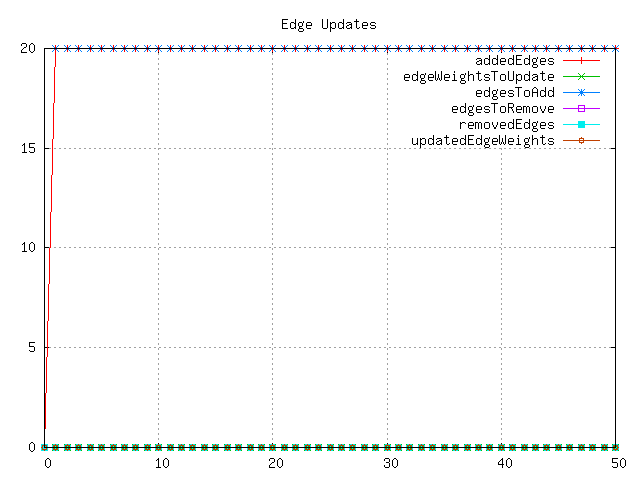
\includegraphics [scale=0.8] {plots/z.statistics.updates.edges}
	\caption{z.statistics.updates.edges}
	\label{plot:RANDOM_100_500 - BARABASI_ALBERT_GROWTH_10_2.z.statistics.updates.edges}
\end{figure}

% plot z.statistics.updates.edges.CDF
\begin{figure} [h]
	\centering
	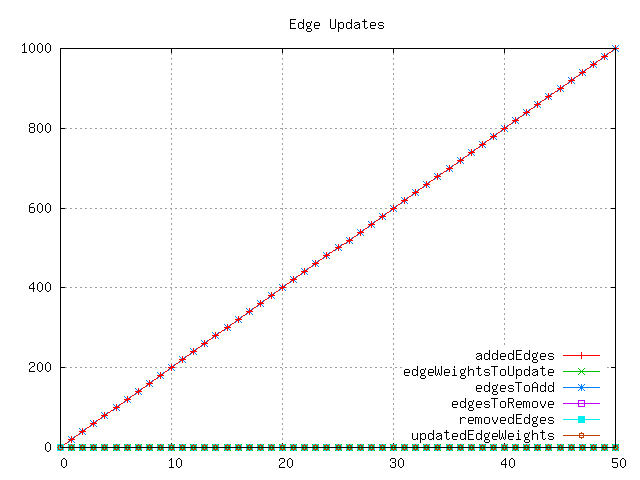
\includegraphics [scale=0.8] {plots/z.statistics.updates.edges.CDF}
	\caption{z.statistics.updates.edges.CDF}
	\label{plot:RANDOM_100_500 - BARABASI_ALBERT_GROWTH_10_2.z.statistics.updates.edges.CDF}
\end{figure}

% plot z.statistics.updates.nodes
\begin{figure} [h]
	\centering
	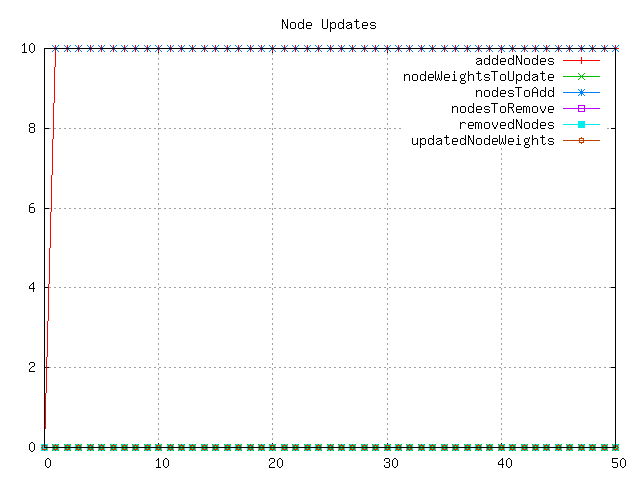
\includegraphics [scale=0.8] {plots/z.statistics.updates.nodes}
	\caption{z.statistics.updates.nodes}
	\label{plot:RANDOM_100_500 - BARABASI_ALBERT_GROWTH_10_2.z.statistics.updates.nodes}
\end{figure}

% plot z.statistics.updates.nodes.CDF
\begin{figure} [h]
	\centering
	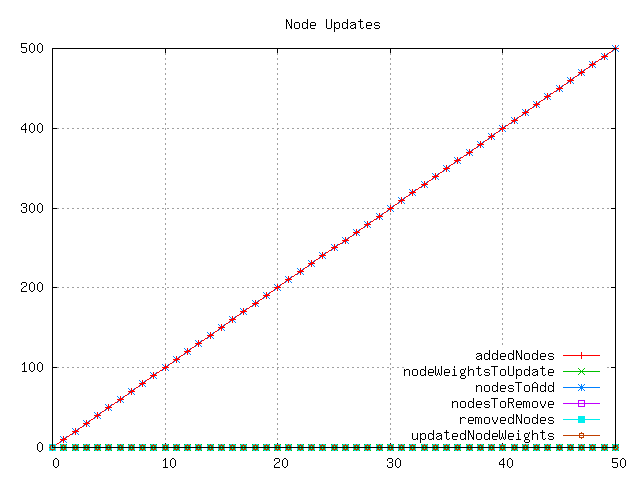
\includegraphics [scale=0.8] {plots/z.statistics.updates.nodes.CDF}
	\caption{z.statistics.updates.nodes.CDF}
	\label{plot:RANDOM_100_500 - BARABASI_ALBERT_GROWTH_10_2.z.statistics.updates.nodes.CDF}
\end{figure}

% plot z.statistics.memory
\begin{figure} [h]
	\centering
	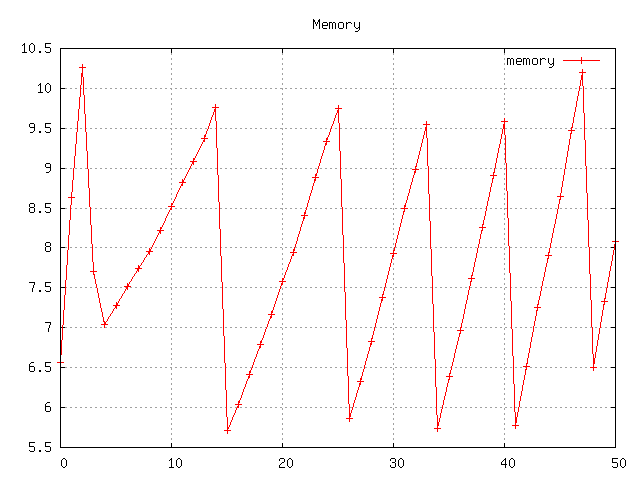
\includegraphics [scale=0.8] {plots/z.statistics.memory}
	\caption{z.statistics.memory}
	\label{plot:RANDOM_100_500 - BARABASI_ALBERT_GROWTH_10_2.z.statistics.memory}
\end{figure}

% plot z.statistics.edges
\begin{figure} [h]
	\centering
	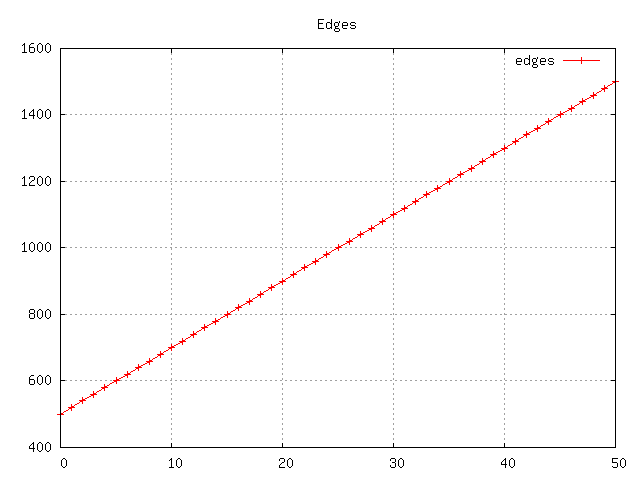
\includegraphics [scale=0.8] {plots/z.statistics.edges}
	\caption{z.statistics.edges}
	\label{plot:RANDOM_100_500 - BARABASI_ALBERT_GROWTH_10_2.z.statistics.edges}
\end{figure}

% plot z.statistics.nodes
\begin{figure} [h]
	\centering
	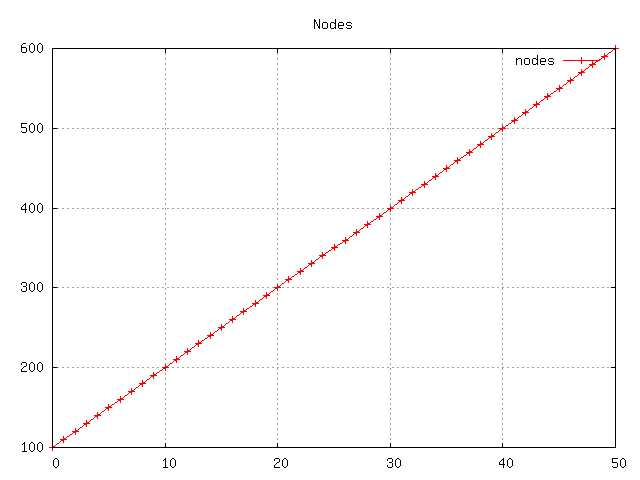
\includegraphics [scale=0.8] {plots/z.statistics.nodes}
	\caption{z.statistics.nodes}
	\label{plot:RANDOM_100_500 - BARABASI_ALBERT_GROWTH_10_2.z.statistics.nodes}
\end{figure}


% end of document
